% $Id: INF_Poster_example.tex 7714 2011-08-31 17:34:46Z tkren $
%
% TU Wien - Faculty of Informatics
% poster template
%
% This template is using the beamer document class and beamerposter package, see
% <http://www.ctan.org/tex-archive/macros/latex/contrib/beamer/>
% <http://www.ctan.org/tex-archive/macros/latex/contrib/beamerposter/>
% <http://www-i6.informatik.rwth-aachen.de/~dreuw/latexbeamerposter.php>
%
% For questions and comments send an email to
% Thomas Krennwallner <tkren@kr.tuwien.ac.at>
%

\documentclass[final,hyperref={pdfpagelabels=true}]{beamer}

\usepackage{TUINFPST}
\usepackage{comment}
\usepackage{tabularx}
\usepackage{mathdots} % makes vdots scale properly

\usepackage{lipsum}
\usepackage{graphicx, array, blindtext}


\newcommand*{\tabbox}[2][t]{%
	    \vspace{0pt}\parbox[#1][3.7\baselineskip]{1cm}{\strut#2\strut}}



%\title[Computational Intelligence]{Interactive Computer Generated Architecture}
% if you have a long title looking squeezed on the poster, just force
% some distance:
\title[Computational Intelligence]{%
	Interpolation in First-Order Logic
	\\[0.2\baselineskip]%
	with Equality
	%\\[0.2\baselineskip]%
}
%\author[b.mallinger@gmx.at]{Bernhard Mallinger}
\author[b.mallinger@gmx.at]{Bernhard Mallinger}
\institute[]{%
	Technische Universit{\"a}t Wien\\[0.25\baselineskip]
	Institut f{\"u}r diskrete Mathematik und Geometrie\\[0.25\baselineskip]
	Forschungsgruppe: Computational Logic\\[0.25\baselineskip]
	Betreuer: Ass.Prof.\ Stefan Hetzl
}
%\titlegraphic{ {\Huge \color{red} TODO:~LOGO}
\includegraphics[height=52mm]{logo_KBS_2_CMYK}}
\date[\today]{\today}
\subject{epilog}
%\keywords{my kwd1, my kwd2}

%%%%%%%%%%%%%%%%%%%%%%%%%%%%%%%%%%%%%%%%%%%%%%%%%%%%%%%%%%%%%%%%%%%%%%%%%%%%%%%%%%%%%%

% Display a grid to help align images 
%\beamertemplategridbackground[12.7mm]

% play around with the background colors
% \setbeamercolor{background canvas}{bg=yellow}

% use a background picture
% \usebackgroundtemplate{%
%   
\includegraphics[width=\paperwidth]{logo_KBS_2_CMYK}
% }

\newcommand{\colOne}[1]{ {\color{TuInfRed}#1}}
\newcommand{\colTwo}[1]{ {\color{TuWienBlue}#1}}

\newcommand{\colA}[1]{ \colOne{#1} }
\newcommand{\colB}[1]{ \colTwo{#1} }


%\definecolor{darkgray}{rgb}{0.4, 0.4, 0.4}
\newcommand{\gray}[1]{ {\color{InfosysDarkGrey}#1}}

% play around with block colors
\setbeamercolor{block body}{fg=black,bg=white}
\setbeamercolor{block title}{fg=TuWienBlue,bg=white}

\setbeamertemplate{block begin}{
	\begin{beamercolorbox}{block title}%
		\begin{tikzpicture}%
			\node[draw,rectangle,line width=3pt,rounded corners=0pt,inner sep=0pt]{%
				\begin{minipage}[c][2cm]{\linewidth}
					\centering\textbf{\insertblocktitle}
				\end{minipage}
			};
		\end{tikzpicture}%
	\end{beamercolorbox}
	\vspace*{1cm}
	\begin{beamercolorbox}{block body}%
	}

	\setbeamertemplate{block end}{
	\end{beamercolorbox}
	\vspace{2cm}
}


% http://tikz.de/zweifarbige-buchstaben/
\tikzset{
   bclleft/.style={.},
   letter left/.style={bclleft/.append style={#1}},
   bclright/.style={.},
   letter right/.style={bclright/.append style={#1}},
}
\newcommand\bicolorletter[2][]{%
   \tikz[baseline=(n.base),inner sep=0pt,outer xsep=0pt,#1]{
     \node(n){\phantom{#2}};
     \foreach \a/\c in {west/bclleft,east/bclright}{
       \begin{scope}
         \clip(n.south)rectangle(n.north \a);
				 \node[\c]at(n){${#2}$};
				 %\node[\c]at(n){\textrm{#2}};
       \end{scope}
     }}}

\newcommand{\myA}{ \tikzset{letter left=InfosysDarkGrey,letter right=TuInfRed} \bicolorletter{A} }
\newcommand{\myB}{ \tikzset{letter left=InfosysDarkGrey,letter right=TuWienBlue} \bicolorletter{B} }

\usepackage{trimclip,xcolor}

\newcommand{\Atwo}{%
  \mbox{%
    \def\Ahalf##1{\dimexpr.5\width ##1 -0.065em\relax}
   	\textcolor{InfosysDarkGrey}{\clipbox{0 0 {\Ahalf+} 0}{$A$}}%
    \textcolor{TuInfRed}{\clipbox{{\Ahalf-} 0 0 0}{$A$}}%
   	%\textcolor{TuInfRed}{\clipbox{0 0 {\Ahalf+} 0}{$A$}}%
    %\textcolor{InfosysDarkGrey}{\clipbox{{\Ahalf-} 0 0 0}{$A$}}%
  }%
}
%\newcommand{\myA}{ \Atwo }



% setup postit
\setbeamercolor{postit}{fg=black,bg=yellow} 
\newenvironment{postit}
{\begin{beamercolorbox}[sep=1em,wd=7cm]{postit}}
{\end{beamercolorbox}}

\usepackage{tikz}
\usetikzlibrary{shapes,arrows,backgrounds,graphs,%
	matrix,patterns,arrows,decorations.pathmorphing,decorations.pathreplacing,%
	positioning,fit,calc,decorations.text,shadows,decorations.markings%
}


%\usepackage{amsmath}
%\usepackage{amsthm}
%\usepackage{amssymb} % the reals
%\usepackage{mathtools} % smashoperator
%\usepackage{thmtools} 

%\usepackage{MnSymbol} % again other symbols

\newcommand{\itemizeOnBlockStart}{
		\vspace*{-0.5em}
	}


\newcommand{\entails}{\vDash}
\newcommand{\notentails}{\nvDash}
\newcommand{\proves}{\vdash}

\DeclareMathOperator{\limpl}{\supset}
\DeclareMathOperator{\liff}{\lra}
\DeclareMathOperator{\semiff}{\Lra}
\newcommand{\syneq}{\equiv}
\newcommand{\union}{\cup}
\newcommand{\bigunion}{\bigcup}
\newcommand{\intersection}{\cap}
\newcommand{\bigintersection}{\bigcap}
\newcommand{\intersect}{\intersection}
\newcommand{\bigintersect}{\bigintersection}





%\declaretheorem[title=Theorem]{thm}

\newcommand{\contrib}[1]{{\color{TuWienBlue}\textbf{#1}}}

% for crop marks, uncomment the following line
%\usepackage[cross,width=88truecm,height=123truecm,center]{crop}

%%%%%%%%%%%%%%%%%%%%%%%%%%%%%%%%%%%%%%%%%%%%%%%%%%%%%%%%%%%%%%%%%%%%%%%%%%%%%%%%%%%%%%

\begin{document}

% We have a single poster frame.
\begin{frame}
	\begin{columns}[t]

		%\newcommand{\mycolwidth}{.4\textwidth} % default: .45\textwidth
		\newcommand{\mycolwidth}{.45\textwidth} 

		\begin{column}{\mycolwidth}

			\begin{block}{Craig Interpolation}



				\textbf{Theorem} (Craig).
				\emph{
					Let \myA{} 
					and \myB{} be first-order formulas 
					such that $\entails \myA\supset \myB$ where \myA{} contains \colA{red} and \gray{gray} symbols and \myB{} contains of \colB{blue} and \gray{gray} symbols.
					%Let \myA{} be a first-order formula consisting of \colA{red} and \gray{gray} symbols 
					%and \myB{} a first-order formula consisting of \colB{blue} and \gray{gray} symbols 
					%such that $\entails \myA\supset \myB$.
					Then there is an interpolant $\gray I$ containing of \gray{gray} symbols  for $\myA$ and~$\myB$ such that:
					\begin{itemize}
						\item $\entails \myA \limpl \gray I$
						\item $\entails \gray I \limpl \myB$
						%\item $\operatorname{Lang}(\gray I) \subseteq
						%	\operatorname{Lang}(\myA) \cap \operatorname{Lang}(\myB)$
					\end{itemize}
				}
				\vspace{1em}


				\begin{figure}[htbp]
					\centering
					\begin{tikzpicture}[
							implies/.style={double,double equal sign distance,-implies},
							mynode/.style={circle,outer sep=3pt}
						]
						\node[mynode] (A) at (0,0) {$\myA$};
						\node[mynode] (B) at (16,0) {$\myB$};
						\node[mynode] (I) at (8,-6) {$\gray I$};

						%\draw[->,implies] (A) to (B);
						\draw (A) edge[implies]  (B);
						\draw (A) edge[implies]  (I);
						\draw (I) edge[implies]  (B);

					\end{tikzpicture}
					\label{fig:interpol}
					%\caption{Given two formulas $A$ and $B$ such that $A$ implies $B$, an interpolant is a formula $I$ which is implied by $A$ and which implies $B$.}
				\end{figure}
				\vspace{1em}

				$\Rightarrow$ Interpolants give a concise logical summary of the implication

			\end{block}

			\begin{block}{Applications of Craig Interpolation} 
				Theoretical:
				\begin{itemize}
					\item Proof of Beth's Definability Theorem
				\end{itemize}
				Practical:
				\begin{itemize}
					\item Program analysis: Detect loop invariants
					\item Model checking: Overapproximate set of reachable states %of program % saves 1 line
				\end{itemize}
			\end{block}


			\begin{block}{Aim and Scope of the Thesis}
				Give comprehensive account of existing techniques and extend them:
				\begin{itemize}
					\item Model-theoretic proof 
					\item Reduction to first-order logic without equality
					\item Interpolant extraction from resolution proofs
				\end{itemize}
			\end{block}

			\begin{block}{Model-theoretic proof}
				\itemizeOnBlockStart

				\begin{itemize}
					\item Non-constructive proof:
						\begin{itemize}
							\item Let $T_{\myA}$ and $T_{\lnot \myB}$ be theories extending $\myA$ and $\lnot \myB$
							\item Build model from maximal consistent intersection of $T_{\myA}$ and $T_{\lnot \myB}$

								(assuming the non-existence of interpolants)

								$\Rightarrow$ $\myA \land \lnot \myB$ satisfiable
						\end{itemize}
					\item Related to Robinson's Joint Consistency Theorem
				\end{itemize}

			\end{block}


			\begin{block}{Reduction to first-order logic without equality \cite{Craig57linear}} 
				\itemizeOnBlockStart
				%Approach by Craig in \cite{Craig57linear}, 
				\newcommand{\transformsep}{\;\to\;}
				\begin{align*}
					\intertext{Translate equality and function symbols:}
					%\gray P(\colA c) & \transformsep \exists x (\colA C(x) \land \gray P(x)) \\
					\Big(\gray P(\colA c)\Big)^*  & \, \equiv \, \exists x (\colA C(x) \land \gray P(x)) \\
					%\gray P(\colB f( \colA c)) & \transformsep  \exists x (  \exists y( \colA C(y) \land \colB F(y, x)) \land \gray P(x)) \\
					\Big( \gray P(\colB f( \colA c)) \Big)^* & \, \equiv \, \exists x (  \exists y( \colA C(y) \land \colB F(y, x)) \land \gray P(x)) \\
					%\gray s = \gray t & \transformsep \gray E(\gray s, \gray t) \\
					\Big( \gray s = \gray t \Big)^* & \, \equiv \, \gray E(\gray s, \gray t) \\
					\intertext{Add theory of equality:} 
					\varphi & \transformsep T_E \limpl \varphi^*
				\end{align*}
			%\begin{align*}
			%		\intertext{Translate equality and function symbols:}
			%		%\gray P(\colA c) & \transformsep \exists x (\colA C(x) \land \gray P(x)) \\
			%		(\gray P(\colA c))^*  & \, \equiv \, \exists x (\colA C(x) \land \gray P(x)) \\
			%		%\gray P(\colB f( \colA c)) & \transformsep  \exists x (  \exists y( \colA C(y) \land \colB F(y, x)) \land \gray P(x)) \\
			%		( \gray P(\colB f( \colA c)) )^* & \, \equiv \, \exists x (  \exists y( \colA C(y) \land \colB F(y, x)) \land \gray P(x)) \\
			%		%\gray s = \gray t & \transformsep \gray E(\gray s, \gray t) \\
			%		( \gray s = \gray t )^* & \, \equiv \, \gray E(\gray s, \gray t) \\
			%		\intertext{Add theory of equality:} 
			%		\varphi & \transformsep T_E \limpl \varphi^*
			%	\end{align*}


				$\Rightarrow$ Then calculate interpolant in reduced logic

			\end{block}

		\end{column}
		\begin{column}{\mycolwidth}

			% for 0.2\textwidth need 10.35 em
			% 0.18 -> 10.0

					\newcommand{\proofwidth}{0.2\textwidth}
					\newcommand{\proofindent}{\hspace*{10.21em}}
					%\newcommand{\proofwidth}{0.18\textwidth}
					%\newcommand{\proofindent}{\hspace*{10em}}

					%\newcommand{\stagearrow}{{\Large$\Downarrow$}}
					\newcommand{\stagearrow}{{\Large$\Downarrow$}}

			\begin{block}{Interpolant extraction from proofs in two phases \cite{Huang95}}
				%\itemizeOnBlockStart
				%\begin{itemize}
				%	\item Extract structure from proof 
				%	\item Replace colored terms by quantified variables 
				%\end{itemize}

				%\begin{tabular}{*{2}{m{0.48\textwidth}}}
				%	\begin{center}
				%		Proof: 
				%		&
				%		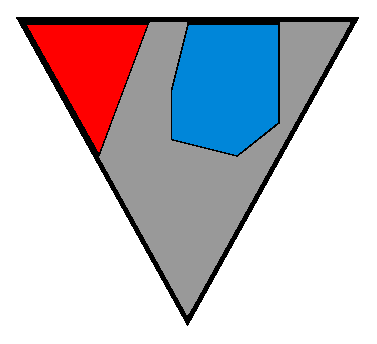
\includegraphics[width=0.2\textwidth]{figures/two_phase_draft_proof}
				%		%\rule{0.4\textwidth}{0.1\textwidth}
				%	\end{center}
				%	&


				%\begin{tabular}{*{4}{m{0.48\textwidth}}}
					\newcommand{\fakemulticolwidth}{0.28\textwidth}
					%\begin{tabularx}{\textwidth}{p{0.25\textwidth}p{0.2\textwidth}l}
					%\begin{tabular}{p{0.25\textwidth}p{0.35\textwidth}c}
					\begin{tabular}{p{0.25\textwidth}ll}

					Proof: 
					&
					%\begin{center}

					\multicolumn{1}{m{\fakemulticolwidth}}{
						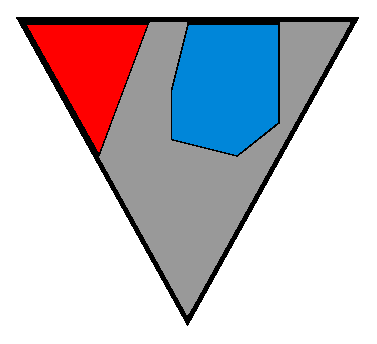
\includegraphics[width=\proofwidth]{figures/two_phase_draft_proof}
					}
					%\rule{0.4\textwidth}{0.1\textwidth}
					%\end{center}
					&
						\vspace*{0.5em}
					\\

				%& \begin{center} \large\stagearrow \end{center} & 
					%\multicolumn{2}{c}{\emph{Extract structure from proof}}
					\multicolumn{2}{l}{
						\proofindent{\stagearrow} ~\parbox[c]{12em}{\emph{ Extract propositional interpolant structure from proof}}
						\vspace*{0.5em}
				}
				 \\
			 
					%&  \Huge\stagearrow}   \\

				\begin{tabular}[x]{@{}l@{}}Propositional\\Interpolant:\end{tabular} 
					%	Propositional \newline interpolant: 
					&
					%\begin{center} \end{center}
					%\rule{0.4\textwidth}{0.1\textwidth}
					\multicolumn{1}{m{\fakemulticolwidth}}{
						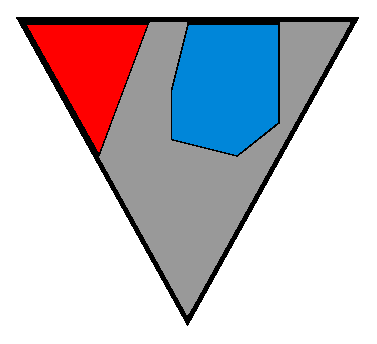
\includegraphics[width=\proofwidth]{figures/two_phase_draft_proof}
					}
					$\dots \gray Q(\colA f(\colB c), \colB c) \dots$
						\vspace*{0.5em}
					\\

	\multicolumn{2}{l}{
						\proofindent{\stagearrow} ~\parbox[c]{12em}{\emph{ Replace colored function and constant symbols }}
						\vspace*{0.5em}
				}
				 \\

				\begin{tabular}[x]{@{}l@{}}Prenex\\First-Order\\Interpolant:\end{tabular} 
					&
					\multicolumn{1}{m{\fakemulticolwidth}}{
						
\includegraphics[width=\proofwidth]{figures/two_phase_draft_fo_interpolant}
					}
					$\exists {x_3} \forall {x_5} \dots \gray Q({x_5}, {x_3}) \dots$
					\\



					\end{tabular}
			\end{block}

			\begin{block}{Interpolant extraction from proofs in one phase}

				%\begin{tabular}{*{4}{m{0.48\textwidth}}}
					\newcommand{\fakemulticolwidth}{0.28\textwidth}
					%\begin{tabularx}{\textwidth}{p{0.25\textwidth}p{0.2\textwidth}l}
					%\begin{tabular}{p{0.25\textwidth}p{0.35\textwidth}c}
					\begin{tabular}{p{0.25\textwidth}ll}

					Proof: 
					&
					%\begin{center}

					\multicolumn{1}{m{\fakemulticolwidth}}{
						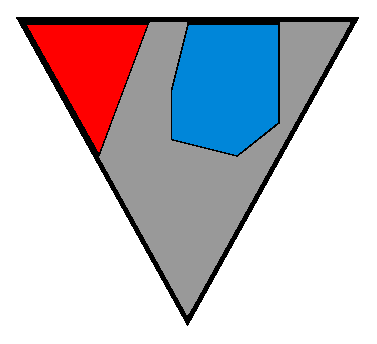
\includegraphics[width=\proofwidth]{figures/two_phase_draft_proof}
					}
					%\rule{0.4\textwidth}{0.1\textwidth}
					%\end{center}
					&
						\vspace*{0.5em}
					\\

				%& \begin{center} \large\stagearrow \end{center} & 
					%\multicolumn{2}{c}{\emph{Extract structure from proof}}
					\multicolumn{2}{l}{
						\proofindent
						$\left.
						\parbox[c]{2em}{
							\stagearrow\\
							\hspace*{0.318em}$\vdots$ \\[0.27\baselineskip]
							\stagearrow
						}
					\right\} 
					\parbox[t]{11em}{\emph{Combined extraction and replacing phases}}
					$
						\vspace*{0.5em}
					} 
				 \\
			 
					%&  \Huge\stagearrow}   \\

				%\begin{tabular}[x]{@{}l@{}}Intermediate\\Formula:\end{tabular} 
					%	Propositional \newline interpolant: 
					&
					%\begin{center} \end{center}
					%\rule{0.4\textwidth}{0.1\textwidth}
					\multicolumn{1}{m{\fakemulticolwidth}}{
						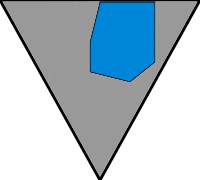
\includegraphics[width=\proofwidth]{figures/one_phase_draft_intermediate}
					}
					$\dots \forall {x_5} \dots \gray Q({x_5}, \colB c) \dots$
						\vspace*{0.5em}
					\\
					\multicolumn{2}{l}{
						\proofindent
						$\left.
						\parbox[c]{2em}{
							\stagearrow\\
							\hspace*{0.318em}$\vdots$ \\[0.27\baselineskip]
							\stagearrow
						}
					\right\} 
					\parbox[t]{11em}{\emph{Combined extraction and replacing phases}}
					$
						\vspace*{0.5em}
					} 
				 \\

				\begin{tabular}[x]{@{}l@{}}Non-Prenex\\First-Order\\Interpolant:\end{tabular} 
					&
					\multicolumn{1}{m{\fakemulticolwidth}}{
						
\includegraphics[width=\proofwidth]{figures/two_phase_draft_fo_interpolant}
					}
					$\exists {x_3} \dots \forall {x_5} \dots \gray Q({x_5}, {x_3}) \dots$
					\\



					\end{tabular}
			\end{block}


				


			\begin{block}{Contributions}
			\itemizeOnBlockStart
				\begin{itemize}
					\item We introduced the one phase extraction approach.
					\item We showed that the number of quantifier alternations in the interpolant corresponds to the number of color alternations in terms.

				\end{itemize}

			\end{block}

			\setbeamertemplate{bibliography item}{\insertbiblabel}

			\begin{block}{References}
			\itemizeOnBlockStart
				\definecolor{lightviolet}{cmyk}{0.19,0.21,0,0.31}

				% this is just an example, use BibTeX!
				\begin{thebibliography}{999}
						%\setbeamertemplate{bibliography item}{[1]}

					\bibitem[1]{Craig57linear}
						%William Craig.
						%\newblock{
						%	Linear Reasoning. A New Form of the Herbrand-Gentzen Theorem.
						%}
						%\newblock {
						%	\emph{Journal of Symbolic Logic}, 22(3):250--268, 1957.
						%}
						William Craig.
						{
							\color{black}
							Linear Reasoning. A New Form of the Herbrand-Gentzen Theorem.
						}
						{
							%\color{lightviolet}
							\emph{Journal of Symbolic Logic}, 22(3):250--268, 1957.
						}


					\bibitem[2]{Huang95}
						%Guoxiang Huang.
						%\newblock{
						%	Constructing Craig Interpolation Formulas.
						%}
						%\newblock {
						%	%\emph{Proceedings of the First Annual International Conference on Computing and Combinatorics}, COCOON ’95, p.\ 181--190, 1995. 
						%	In \emph{Proc COCOON ’95}, p.\ 181--190, 1995. 
						%}
						Guoxiang Huang.
						{
							\color{black}
							Constructing Craig Interpolation Formulas.
							%\emph{Proceedings of the First Annual International Conference on Computing and Combinatorics}, COCOON ’95, p.\ 181--190, 1995. 
						}
						{
							%\color{lightviolet}
							In \emph{Proc COCOON ’95}, p.\ 181--190, 1995. 
						}



						%  \newblock {On logical representations of hackerisms}.
						%  {\em J.~Log.~Hack.} 1:1--2.

						%	
						%  \bibitem[Foo~and~Fu, 2010]{ff2010}
						%    Foo, B.; and Fu, B.
						%    2010.
						%    \newblock {On logical representations of hackerisms}.
						%    {\em J.~Log.~Hack.} 1:1--2.
						%    
						%    
						%  \bibitem[Crock~et~al., 2010]{ck2010}
						%    Crock, A; Cruft, B.; and Kludge, C.
						%    2010.
						%    \newblock {Decomposing junk code}.
						%    Manuscript.
						%    
				\end{thebibliography}
			\end{block}
		\end{column}
		% ---------------------------------------------------------%
		% end the column
	\end{columns}

	%\begin{tikzpicture}[remember picture,overlay]
	%	\node[inner sep=0pt,xshift=-30cm,yshift=23cm] at (current page.east) {%
	%		\begin{postit}%
	%			Post-It time!%
	%		\end{postit}%
	%	}; 
	%\end{tikzpicture}

\end{frame}

\end{document}

%%% Local Variables:
%%% TeX-PDF-mode: t
%%% TeX-debug-bad-boxes: t
%%% TeX-master: t
%%% TeX-parse-self: t
%%% TeX-auto-save: t
%%% reftex-plug-into-AUCTeX: t
%%% End:
